\chapter{Metodologie}
\section{Strumenti utilizzati}
Dopo un'accurata attività di ricerca, gli strumenti più adatti allo scopo della tesi si sono rivelati essere Protégé\cite{protege} (un editor per ontologie), ONT2BN\cite{kalet2017} (descritto nel capitolo precedente), e Genie\cite{genie}, un software commerciale per lavorare con reti Bayesiane disponibile anche in versione gratuita per fini accademici.

\section{L'approccio proposto}
\subsection{L'ontologia di partenza}
Al fine di dimostrare il procedimento seguito, verrà riprodotto, a partire da un'ontologia, l'esempio contenuto in [Stella, 2018]\cite{stella2018}, contenente 5 entità: \texttt{Earthquake}, \texttt{Intrusion}, \texttt{Alarm}, \texttt{Mary calls}, \texttt{John calls}. In particolare, a partire dall'esempio (che, in versione originale, consiste in una rete Bayesiana già formata) è stata generata una semplice ontologia che funge da \textit{proof of concept}, successivamente utilizzata per produrre la rete Bayesiana tramite ONT2BN e data in input a Genie.\\
\\Innanzitutto, viene definita la relazione \texttt{dependsOn}:
\begin{lstlisting}[language=xml]
<owl:ObjectProperty rdf:about=``https://soligo.org/ont/test-ontology#dependsOn''>
	<rdfs:subPropertyOf rdf:resource=``http://www.w3.org/2002/07/owl#topObjectProperty''/>
</owl:ObjectProperty>
\end{lstlisting}

\clearpage Successivamente, vengono definite le varie entità, ad esempio \texttt{John\_calls}:
\begin{lstlisting}[language=xml]
<owl:Class rdf:about="https://soligo.org/ont/test-ontology#John_calls">
	<rdfs:subClassOf rdf:resource="https://soligo.org/ont/test-ontology#Action"/>
	<rdfs:subClassOf>
		<owl:Restriction>
			<owl:onProperty rdf:resource="https://soligo.org/ont/test-ontology#dependsOn"/>
			<owl:someValuesFrom rdf:resource="https://soligo.org/ont/test-ontology#Alarm"/>
		</owl:Restriction>
	</rdfs:subClassOf>
	<owl:disjointWith rdf:resource="https://soligo.org/ont/test-ontology#Mary_calls"/>
</owl:Class>
\end{lstlisting}

In questo caso, \texttt{John\_calls} è definito come sottoclasse di \texttt{Action} che dipende da \texttt{Alarm}. 
Inoltre viene affermato che, nel caso lo stato del genitore comune \texttt{Alarm} sia noto, i due figli \texttt{John\_calls} e \texttt{Mary\_calls} sono condizionalmente indipendenti; in caso contrario (stato di \texttt{Alarm} ignoto), i due sono dipendenti.

È bene precisare che la relazione \texttt{owl:disjointWith}, dal punto di vista strettamente ontologico, sta a significare che due classi non possono avere istanze in comune (ad esempio, \texttt{Umano} e \texttt{Cane}): l'interpretazione precedente è già posta in ottica inferenziale tramite rete Bayesiana.


\subsection{La ``conversione''}
La ``conversione'' da ontologia a rete Bayesiana richiede diversi passaggi.

Il primo consiste nell'adattare l'ontologia alla sintassi di ONT2BN, ovvero di tradurre le relazioni di dipendenza in modo che si chiamino tutte \texttt{dependsOnX}, con $1 \le$ \texttt{X} $\le 4$ (oppure \texttt{X} omessa). Per fare ciò viene utilizzato Protégé, che fornisce un'interfaccia semplice per creare ontologie, aggiungervi elementi e stabilire relazioni tra di essi (fig. \ref{fig:protegetestontology}).

\begin{figure}[H]
	\centering
	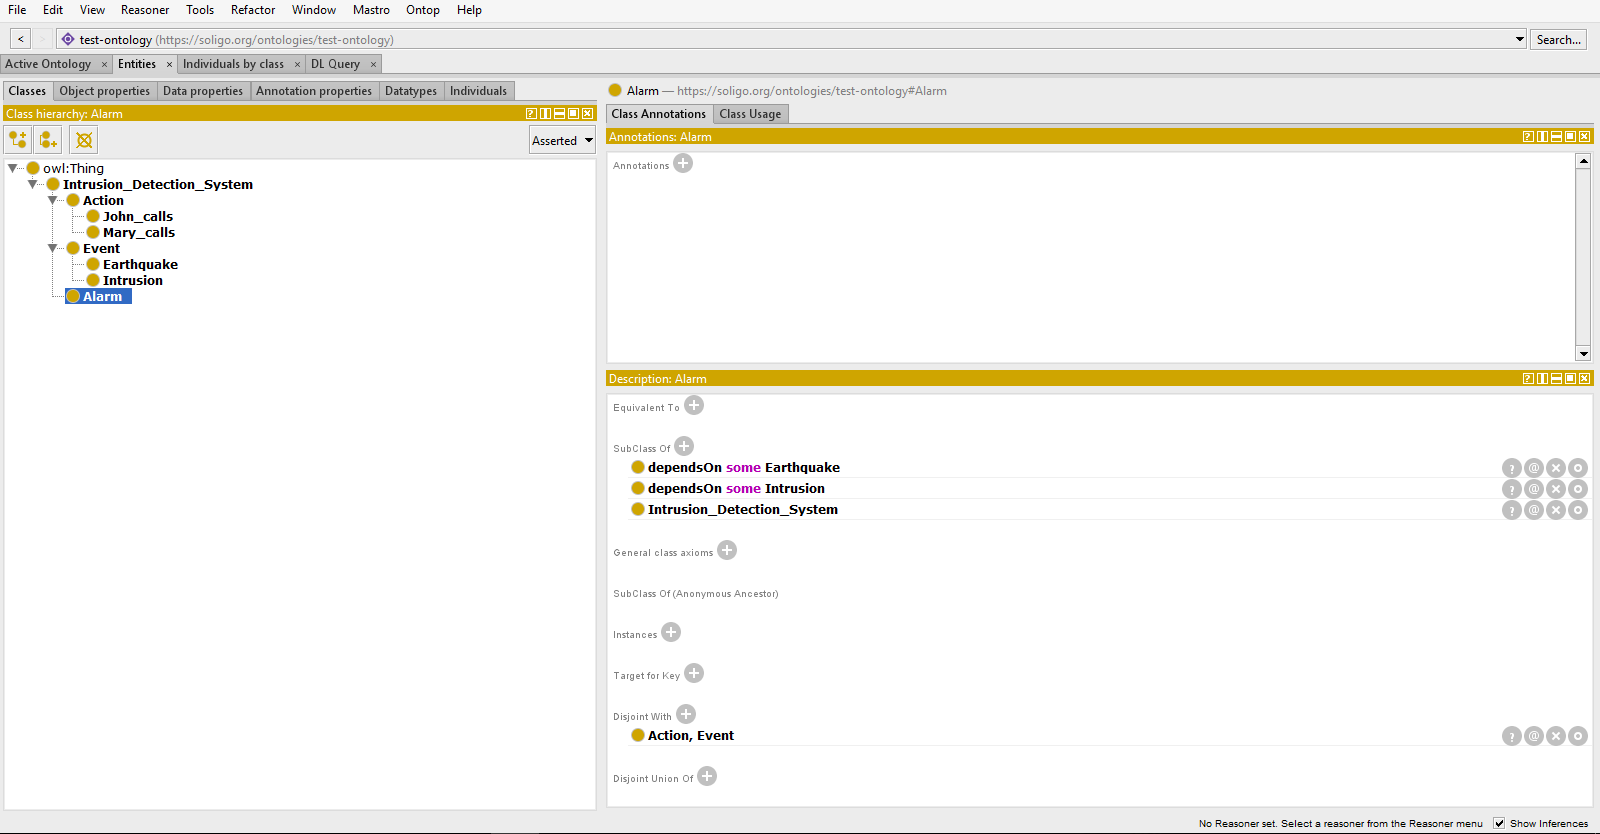
\includegraphics[width=\linewidth]{../images/protege_test_ontology}
	\caption{Ontologia di test in Protégé}
	\label{fig:protegetestontology}
\end{figure}

\clearpage
Successivamente, tramite ONT2BN è fondamentale verificare che gli archi siano orientati correttamente - ed, in caso non lo siano, invertirne la direzione (fig. \ref{fig:ont2bntestontology}). 

\begin{figure}[H]
	\centering
	\includegraphics[width=1\linewidth]{../images/ont2bn_test_ontology}
	\caption{Rete generata a partire dall'ontologia di test con ONT2BN}
	\label{fig:ont2bntestontology}
\end{figure}

Svolta questa operazione, è possibile scaricare l'ontologia in formato \texttt{.net} per Hugin e Genie (fig. \ref{fig:ont2bntestontologydownload}).


\begin{figure}[H]
	\centering
	\includegraphics[width=1\linewidth]{../images/ont2bn_test_ontology_download}
	\caption{Download della rete in formato .net da ONT2BN}
	\label{fig:ont2bntestontologydownload}
\end{figure}

Infine, è possibile importare la rete in Genie, che consente di assegnare valori di probabilità ai vari nodi (ovvero definire le CPT) e svolgere inferenze (fig. \ref{fig:genietestontologyinf}).

\begin{figure}[H]
	\centering
	\includegraphics[width=1\linewidth]{../images/genie_test_ontology_inf}
	\caption{Inferenza sulla rete importata in Genie}
	\label{fig:genietestontologyinf}
\end{figure}


\section{Prima analisi dei risultati}
Questo semplice esempio dimostra come sia possibile passare da un'ontologia ad una rete Bayesiana con pochi passaggi. 

Gli strumenti utilizzati, se correttamente coordinati come specificato, funzionano come previsto e rendono la ``conversione'' un procedimento piuttosto veloce e potente. 

In particolare: Protégé semplifica la creazione da zero e l'elaborazione di ontologie; ONT2BN offre un'interfaccia intuitiva per lavorare sulla rete generata; Genie offre enormi potenzialità dal punto di vista inferenziale.

Purtroppo, rimangono evidenti limiti nella procedura esposta.

Come già detto, la presenza di un esperto che aiuti a selezionare che entità mantenere o eliminare e ad orientare gli archi nella rete Bayesiana è fondamentale: in primis, per rappresentare correttamente i fattori influenti ai fini diagnostici; in secondo luogo, per riuscire a catturare ed esprimere le giuste relazioni di dipendenza causale. 

È anche raro che un'ontologia abbia solo relazioni \texttt{dependsOn}: questo rende necessario effettuare una serie di modifiche che, sebbene non invasive, risultano comunque essere un possibile ostacolo; è anche piuttosto complesso (e, forse, limitante) esprimere tutte le complesse dipendenze di un dominio con la sola relazione \texttt{dependsOn}. 

È già possibile intuire come, sebbene la procedura proposta sia adeguata al fine da raggiungere, siano necessari ancora numerosi sforzi di ricerca per risolvere le problematiche presentate.